\chapter{Preliminary}

\setcounter{page}{1}
\pagenumbering{arabic}

\section{Statistical Depth}
The concept of statistical depth was introduced in order to overcome the lack of a canonical ordering in $\mathbb{R}^d$ for $d > 1$, hence the absence of the related notions of quantile and distribution functions, ranks and signs. The earliest and most popular depth concept is \textit{\textcolor{magenta}{Tukey's halfspace depth}} (see \cite{tukey1975mathematics}).
\begin{definition}
Let $\mathrm{X} = \{x_1, x_2, \dots, x_n\}$ be a finite set of data points in $\mathbb{R}^d$ and let $x$ be an abitrary point, not necessary in $X$. The \textit{depth} of $x$ relative to $X$ is defined as the samllest number of points of $X$ lying in any closed halfspace determined by a line through $x$ (see Figure \ref{fg: depth} from \cite{miller2003efficient}).
\end{definition}

\begin{figure}
	\centering
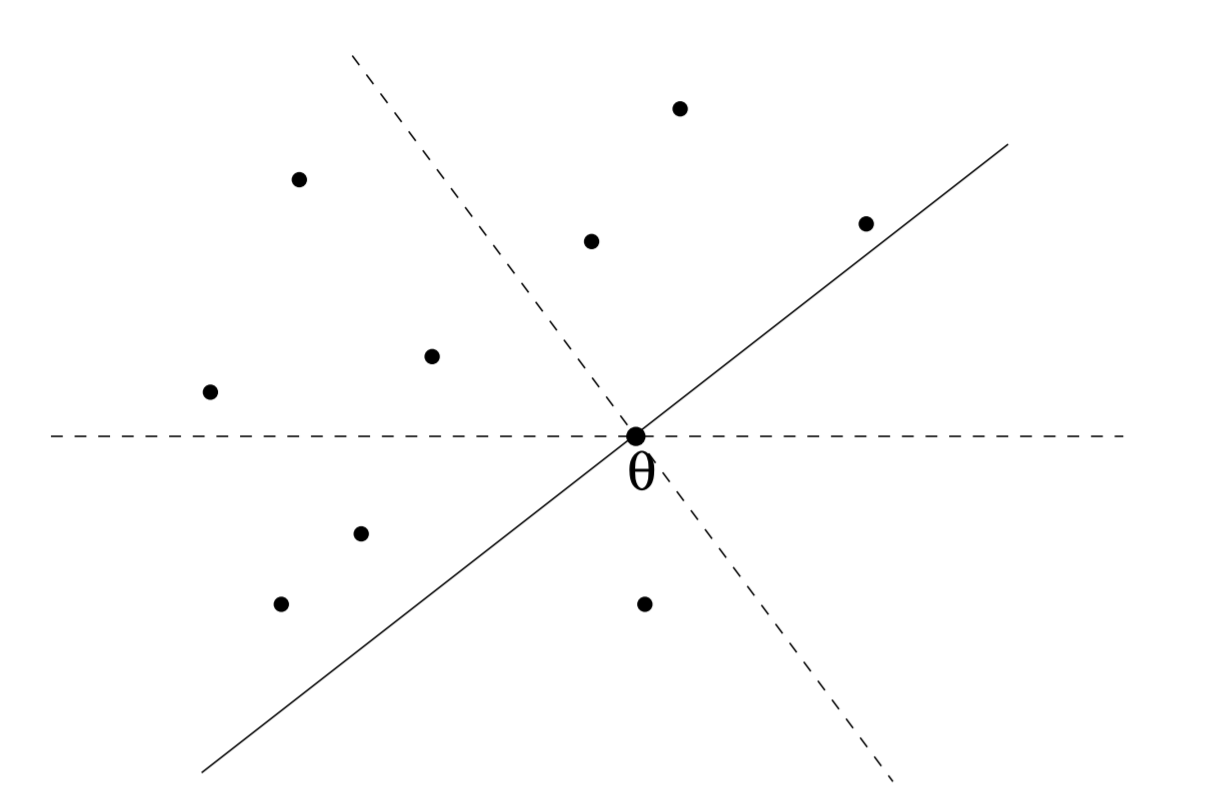
\includegraphics[width=0.5\textwidth]{Figures/IntuitionDepth.png}
\caption{The point $x$ (which is not a data point) as depth $1$.}
\label{fg: depth}
\end{figure}
\begin{remark}
	In detail, the halfspace depth $D_{P}^{Tukey}(x)$ can be written as 
	\begin{IEEEeqnarray}{rCl}
		D_{P}^{Tukey}(x) & \triangleq & \min_{\phi \in \mathcal{S}^{d-1}} \# \left\{ i : \left(x_i - x\right)^T \phi \geq 0 \right\}, \nonumber
	\end{IEEEeqnarray}
where $\mathcal{S}^{d-1}$ denotes the the unit sphere in $\mathbb{R}^d$. 
\end{remark}
\begin{remark}
	It can be seen that the more $x$ is centrally located, the higher its depth. And the depth can be at most $[n/2]$ when $X$ is symmetric about $x$, e.g., in $1$-d case, the median of $X$ has the largest value of depth. Hence, the depth ordering qualifies as a \textit{\textcolor{magenta}{center-outward ordering}} of points in $\mathbb{R}^d$ relative to the center given by the set of the deeptest points, $\arg\sup\limits_{x \in \mathbb{R}^d}D_P^{Tukey}(x)$. 
\end{remark}

Then Tukey considered the use of \textit{contour} of depth for indicating the shape of two-dimensional datasets.
\begin{definition}
	For a fixed positive integer $k$, the \textit{\textcolor{magenta}{$k$-th depth region}} $\mathbb{C}_P(k)$ is the set of all $x \in \mathbb{R}^d$ with $D_P^{Tukey}(x) \geq k$ (see Figure \ref{fg: contour} from \cite{miller2003efficient}). 
\end{definition}
\begin{figure}
	\centering
	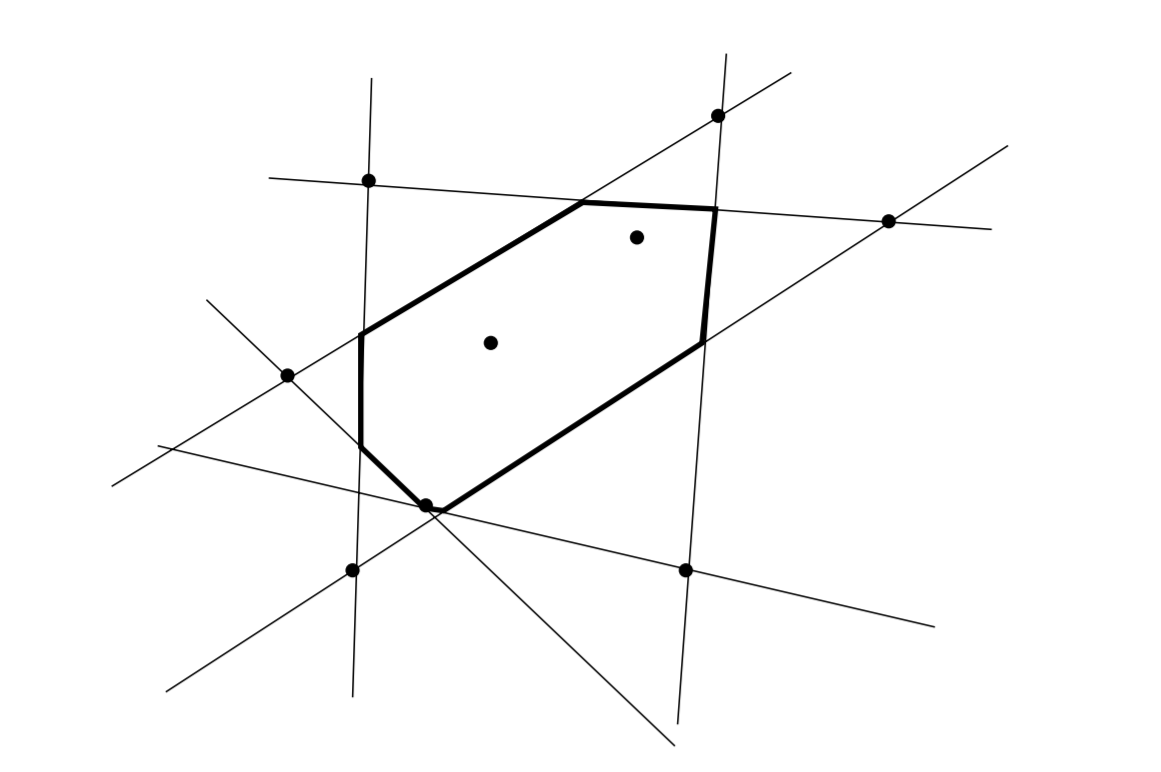
\includegraphics[width=0.5\textwidth]{Figures/IntuitionContour.png}
	\caption{The boundary of depth contour $2$ is drawn in bold.}
	\label{fg: contour}
\end{figure}
\begin{remark}
	By construction, the depth region are nested:
	\[
	\forall (d, d^{\prime}) \in \mathbb{R}^2_+, \quad d^{\prime} \geq d \Rightarrow  \mathbb{C}_P(d^{\prime}) \subset \mathbb{C}_P(d).
	\]
\end{remark}
\begin{remark}
	In fact, $\mathbb{C}_P(k)$ is the intersection of all the $d$-dimensional halfspaces containing $n-k + 1$ points of dataset $X$. In detail,
	\begin{IEEEeqnarray}{rCl}
		\mathbb{C}_P(k) & = & \left\{x \in \mathbb{R}^d : D_P^{Tukey}(x) \geq k\right\} \nonumber \\
		& = & \left\{x \in \mathbb{R}^d : \min_{\phi \in \mathcal{S}^{d-1}} \# \left\{ i : \left(x_i - x\right)^T \phi \geq 0 \right\} \geq k \right\} \nonumber \\
		& = & \bigcap_{\phi \in \mathcal{S}^{d-1} }\left\{x \in \mathbb{R}^d : \# \left\{ i : \left(x_i - x\right)^T \phi \geq 0 \right\} \geq k\right\}.
	\end{IEEEeqnarray}
	Thus, $\mathbb{C}_P(k)$ is convex. This implies that halfspace depth contours \textbf{\textcolor{magenta}{cannot}} pick non-convex features in the geometry of the underlying distribution, as illustrated in Figure \ref{fg: convex}. This feature is shared by most existing depth concepts and might be considered undesirable for distributions with non-convex support.
\end{remark}


\begin{definition}
	For $\tau \in [0, 1]$, \textit{\textcolor{magenta}{the depth region with probability content at least $\tau$}} is 
	\[
	\mathbb{K}_P(\tau) \triangleq \mathbb{C}_P(d(\tau)), \quad d(\tau) \triangleq \sup\{d \in \mathbb{R}: P(\mathbb{C}(d))\geq \tau\}; 
	\]
	the corresponding contour region is the boundary $\mathcal{K}_P(\tau) \triangleq \partial\mathbb{K}_P(\tau)$
\end{definition}
\begin{remark}
	The $d(\tau)$ can be taken as the minimal depth $d$ such that the probability content of $\mathbb{C}_P(d)$ is larger than or equal to $\tau$. Thus for any $x_0 \in \mathbb{K}_P(\tau)$, $x_0$ should lie in the cone.
\end{remark}

\begin{figure}
	\centering
	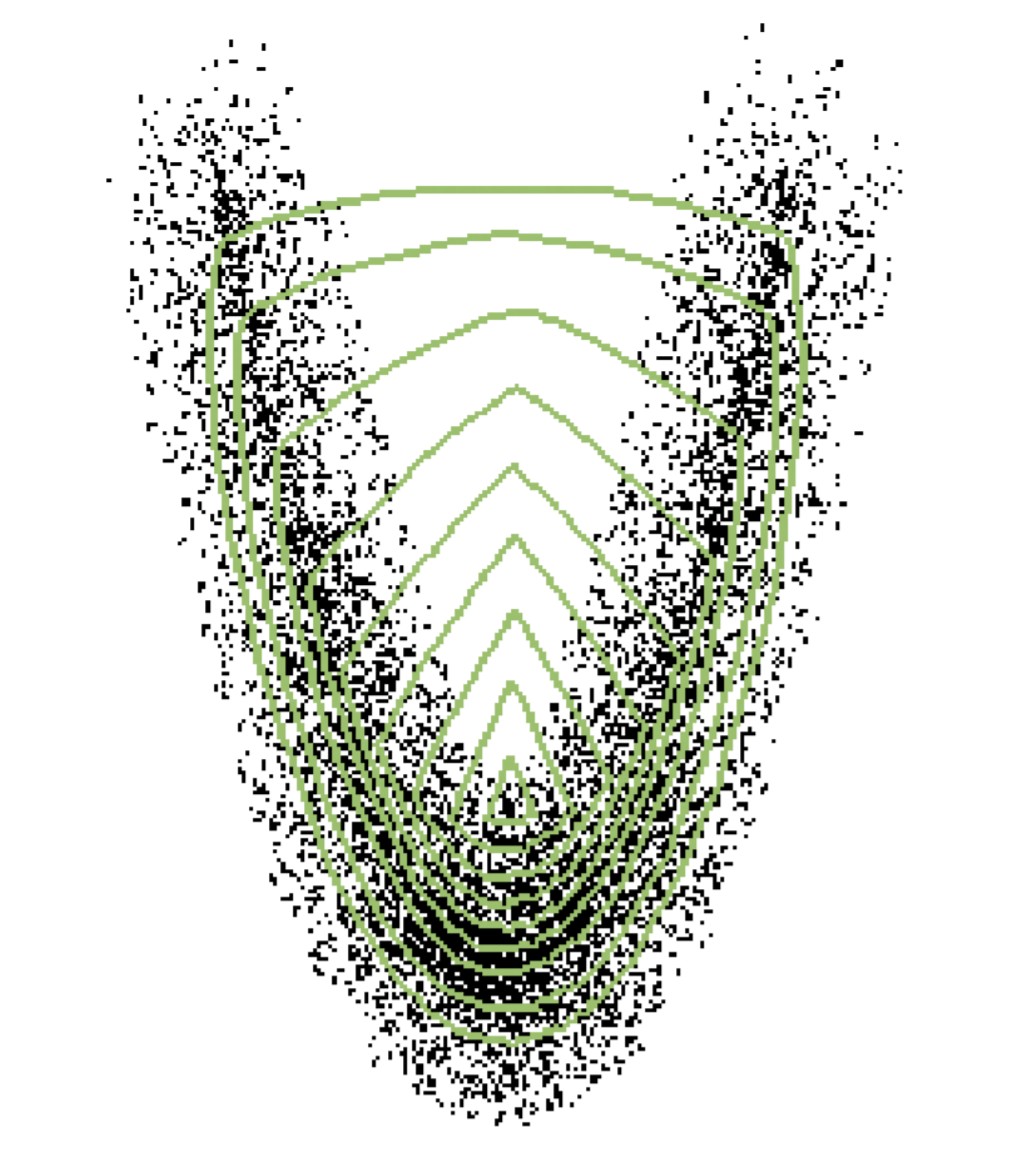
\includegraphics[width=0.5\textwidth]{Figures/Convex.png}
	\caption{Tukey halfspace depth contours for a banana-shaped distribution.}
	\label{fg: convex}
\end{figure} 

\textit{\textcolor{magenta}{Four axioms}} are proposed by \cite{liu1990notion} and \cite{zuo2000general} to unify the diverse depth functions $D_P(x)$:
\begin{itemize}
	\item (Affine invariance) $D_{P_{AX + b}}(Ax + b) = D_{P_X}(x)$, for any $x \in \mathbb{R}^d$, any non-singular $d \times d$ matrix A, and any $b \in \mathbb{R}^d$.
	\item (Maximality at the center) If $x_0$ is a center of symmetry for $P$, it is deepest.
	\item (Linear monotonicity relative to the deepest point) If $x_0$ is deepest, then $D_P(x) \leq D_P((1 - \alpha)x_0 + \alpha x)$ for all $\alpha \in [0, 1]$ 
	\item (Vanishing at infinity) $\lim_{||x|| \to \infty} D_P(x) = 0$.
\end{itemize}

It can be shown that halfspace depth relative to any distribution with non-vanishing density on $\mathbb{R}^d$ satisfies the four axioms above. 

\begin{figure}
	\centering
	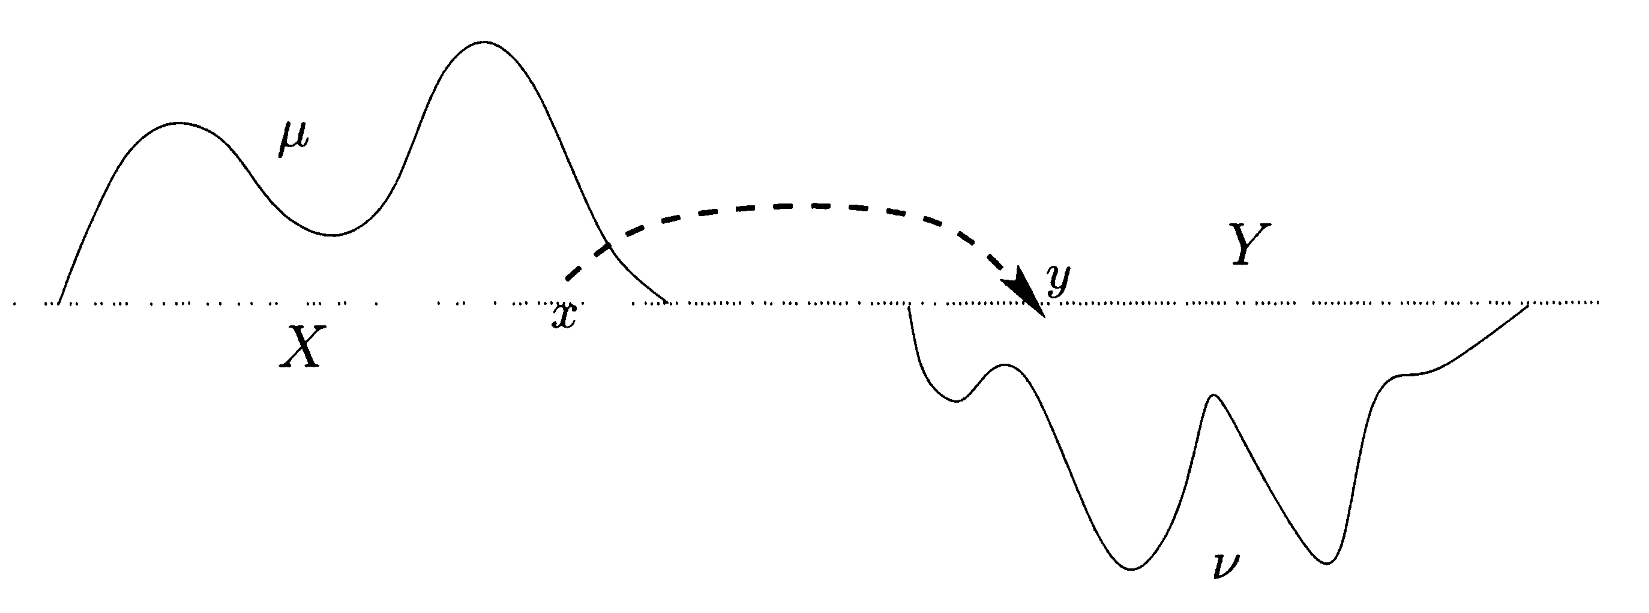
\includegraphics[width = 0.7\textwidth]{Figures/MongePro.png}
	\caption{The Monge's mass transportation problem.}
	\label{fg: monge}
\end{figure}

\section{Optimal Transport}
\subsection{Background and Formulations}
\textbf{Case 1: Monge Problem (Monge formulation)}

Assuming that we are giving a pile of sand, and a hole that we have to completely fill up with the sand. We shall model the pile and the hole with measure space $(X, \mathcal{U}, \mu)$ and $(Y, \mathcal{Y}, \nu)$ respectively (Figure \ref{fg: monge}). Moving the sand around needs some effort, which is modelled by a measurable cost function $c(x, y)$ defined on $X \times Y$. 
\begin{problem}
	We aim to find a measureable \textcolor{magenta}{map} $T : X \to Y$ to minimize 
	\[
	I(T) = \int_{X} c(x, T(x)) d \mu(x), \nonumber
	\]
	under the constrain: $\mu(T^{-1}(A)) = \nu(A)$, for any $A \in \mathcal{Y}$, we shall write as $T\#\mu = \nu$ and say that $\nu$ is the \textit{\textcolor{magenta}{push-forward}} of $\mu$ by $T$.
\end{problem}

\noindent \textbf{Case 2: Mines and Factories (Kantorovich formulation)}

Suppose that we have a collection of $m$ mines mining iron ore and a collection of $n$ factories. We still seek for the most economical way to transport the iron ore to the factories. However, becuase $T$ is a map and the number of mines is not conincide with the number of factories, Monge's formulation is not feasible for this situation. Hence, instead of seeking for a map, we seek for a \textcolor{magenta}{transportation plan}. 

We can use a probability measure $\pi(x, y)$ on the product space $X \times Y$ to model the transport plan. Thus, the problem becomes 
\begin{problem}\label{pro: Kant}
	Minimize 
	\[
	I(\pi) = \int_{X \times Y} c(x, y) d \pi(x, y) \nonumber,
	\]
	where $\pi \in \Pi(\mu, \nu) = \left\{\pi \in P(X \times Y): \mu \ \text{and} \ \nu \ \text{are marginal of} \ \pi \right\}$.
\end{problem}
\begin{remark}
	The set $\Pi(\mu, \nu)$ is not empty, since the tensor produc of $\mu$ and $\nu$ lies in $\Pi(\mu, \nu)$ (this seems to be the most stupid transport plan: every unit sand of $X$, regardless of its location, is distributed over all the factories). In this way, we do not exclude the probability that some mass located at a point $x$ may be split into several parts. 
\end{remark}


\subsection{Kantorovich Duality}
\begin{theorem}\label{th: kan-dual}
	Let $X$ and $Y$ be polish spaces, let $\pi \in P(X \times Y)$, $\mu \in P(X)$ and $\nu \in P(Y)$, and let $c: X \times Y \to \mathbb{R}_+\cup\{+\infty\}$ be a lower semi-continous cost function. Whenever $(\phi, \psi) \in L^1(\mu) \times L^1(\nu)$, define 
	\[
	J(\phi, \psi)=\int_{X} \phi d \mu+\int_{Y} \psi d \nu \nonumber,
	\]
	and
	\[
	\boldsymbol{\Phi}_c = \left\{(\phi, \psi) \in L^1(\mu) \times L^1(\nu): \phi(x)+\psi(y) \leq c(x, y), \ a.s.-\mu, \ a.s.-\nu\right\}.
	\]
	Then
	\begin{IEEEeqnarray}{rCl}
		\inf _{\Pi(\mu, \nu)} I[\pi]=\sup _{\boldsymbol{\Phi_{c}}} J(\phi, \psi) \label{eq: kantDual}
	\end{IEEEeqnarray}
\end{theorem}
\begin{remark}
	Here is an intuitive interpretation of Theorem \ref{th: kan-dual} from \cite{villani2021topics}. Suppose for instance that you are
	both a mathematician and an industrialist, and want to transfer a huge
	amount of coal from your mines to your factories. You can hire trucks to
	do this transportation problem, but you have to pay them $c(x, y)$ for each
	ton of coal which is transported from place $x$ to place $y$. Both the amount
	of coal which you can extract from each mine, and the amount which each
	factory should receive, are fixed. As you are trying to solve the associated
	Monge-Kantorovich problem in order to minimize the price you have to pay,
	another mathematician comes to you and tells you "My friend, let me handle
	this for you: I will ship all your coal with my own trucks and you won't have
	to worry about what goes where. I will just set a price $\phi(x)$ for loading one ton of coal at place $x$, and a price $\psi(y)$ for unloading it at destination $y$. I will set the prices in such a way that your financial interest will be to let me handle all your transportation! Indeed, you can check very easily that for any $x$ and $y$, the sum $\phi(x) + \psi(y)$ will always be less that the cost $c(x, y)$. 
\end{remark}
\begin{proof}
	We can rewrite the left hand side of \ref{eq: kantDual} as
	\begin{IEEEeqnarray}{rCl}
		\inf_{\pi \in \Pi}I(\pi) = \inf_{\pi}\left[I(\pi) + \begin{cases}
			0 & \text{if} \ \pi \in \Pi \\
			+\infty & \text{else}
		\end{cases}\right]. \notag
	\end{IEEEeqnarray}
	Note that 
	\begin{IEEEeqnarray}{rCl}
		\begin{cases}
			0 & \text{if} \ \pi \in \Pi \\
			+\infty & \text{else}
		\end{cases} = \sup_{(\phi, \psi) \in C_b(X) \times C_b(Y) }\left\{\int\phi(x)\md\mu(x) + \int\psi\md\nu(y) - \int \left[\phi(x) + \psi(y)\right] \md \pi(x, y)\right\} \nonumber.
	\end{IEEEeqnarray}
	Thus take \textbf{minimax principle} as grated, we have 
	\begin{IEEEeqnarray}{rCl}
		\inf_{\pi \in \Pi}I(\pi) & = & \inf_{\pi}\sup_{(\phi, \psi) \in C_b(X) \times C_b(Y)}\left[I(\pi) + \int\phi(x)\md\mu(x) + \int\psi\md\nu(y) - \int \left[\phi(x) + \psi(y)\right] \md \pi(x, y)\right] \nonumber \\
		& = & \sup_{(\phi, \psi) \in C_b(X) \times C_b(Y)}\inf_{\pi}\left[\int\phi(x)\md\mu(x) + \int\psi\md\nu(y) -  \int \left[\phi(x) + \psi(y) - c(x, y)\right]\md\pi(x, y)  \right] \nonumber \\
		& = & \sup_{(\phi, \psi) \in C_b(X) \times C_b(Y)}\left\{\int\phi(x)\md\mu(x) + \int\psi\md\nu(y) - \sup_{\pi}\int \left[\phi(x) + \psi(y) - c(x, y)\right]\md\pi(x, y)\right\} \nonumber \\
		& = & \sup_{(\phi, \psi) \in C_b(X) \times C_b(Y)}\left\{J(x, y) - \begin{cases}
			0 & \ \text{if} \ (\phi, \psi) \in \Phi_c \\
			+\infty & \ \text{else} 
		\end{cases}\right\} \nonumber \\
		& = & \sup_{(\phi, \psi) \in \Phi_c}J(x, y) \nonumber.
	\end{IEEEeqnarray}
\end{proof}

Another way to motivate Kantorovich's duality is by analogy with the finite dimensional case (see \cite{evans1997partial}). Firstly, we introduce finite dimensional linear programming by using minimax principle again. 
\begin{example}
	\textbf{Finite dimensional linear programming}
	
	We may prove the following linear programming duality by using minimax principle:
	\begin{IEEEeqnarray}{rCl}
		\sup_{Ax \leq b} c \cdot x & = & \inf_{y \geq 0, A^\top y = c}b \cdot y, \label{eq: finitelinear}
	\end{IEEEeqnarray}
	where $c$ and $b$ are constant vectors in $\mathbb{R}^n$.
	\begin{IEEEeqnarray}{rCl}
		\text{LHS} & = & \sup_{x}\left[c \cdot x + \begin{cases}
			0 & \text{if} \ Ax \leq b \\
			-\infty & \text{else}
		\end{cases}\right] \label{eq: Ex11},
	\end{IEEEeqnarray}
	where we can rewrite function appears inside the bracket as
	\begin{IEEEeqnarray}{rCl}
		\begin{cases}
			0 & \text{if} \ Ax \leq b \\
			-\infty & \text{else}
		\end{cases} & = & \inf_{y \geq 0}\left[y \cdot (b - Ax)\right]. \nonumber
	\end{IEEEeqnarray}
	Thus, we have 
	\begin{IEEEeqnarray}{rCl}
		(\ref{eq: Ex11}) & = & \sup_{x}\left\{c \cdot x + \inf_{y \geq 0}\left[y \cdot (b - Ax)\right] \right\} \nonumber \\
		& = & \sup_{x}\inf_{y \geq 0}\left\{c \cdot x + \left[y \cdot (b - Ax)\right]\right\} \nonumber \\
		& = & \inf_{y \geq 0}\sup_{x}\left\{y \cdot b + c \cdot x - y \cdot(Ax)\right\} \nonumber \\
		& = & \inf_{y \geq 0}\left\{y \cdot b + \sup_{x}\left[(c^\top - y^\top A)x \right]\right\} \nonumber \\
		& = & \inf_{y \geq 0}\left[y \cdot b + \begin{cases}
			0 & \text{if} \ A^\top y = c \\
			+\infty & \text{else}
		\end{cases}\right] \nonumber \\
		& = &  \inf_{y \geq 0, A^\top y = c}b \cdot y. \nonumber
	\end{IEEEeqnarray}
\end{example}
The finite dimensional version of Problem \ref{pro: Kant} can be formulated as follow. Assume $X = \{x_i\}_{i = 1}^n$ and $Y = \{y_i\}_{i = 1}^m$ are two discrete sample spaces with measure $\mu$ and $\nu$, where $\mu_(x_i) = \mu_i$ and $\nu(y_j) = \nu_j$ are positive. And the product space $(X \otimes Y, \mathcal{X} \otimes \mathcal{Y}, \mu \otimes \nu)$, where we define $\mu \otimes \nu (x_i, y_j) = \pi_{ij}$.  Thus, the finite dimensional version of Problem \ref{pro: Kant} can be write as
\begin{IEEEeqnarray}{rCl}
	\min_{\pi_{ij}} \sum\limits_{i = 1}^n\sum\limits_{j = 1}^m c_{ij}\pi_{ij}, \label{eq: finite}
\end{IEEEeqnarray}
under the constraint
\[
\sum\limits_{j = 1}^m\pi_{ij} = \mu_i, \quad \sum\limits_{i = 1}^n \pi_{ij} = \nu_j,
\]
where $c_{ij}$ are postive constants. In fact, this formula can be rewritten as (\ref{eq: finitelinear}), by taking 
\begin{IEEEeqnarray}{rCl}
	b & = & \left(c_{11}, c_{12}, \dots, c_{nm}\right)^\top, \nonumber \\
	y & = & (\pi_{11}, \pi_{12}, \dots, \pi_{nm})^\top, \nonumber \\
	c & = & (\mu_1, \mu_2, \dots, \mu_n, \nu_1, \dots, \nu_m)^\top, \nonumber
\end{IEEEeqnarray}
and 
\begin{equation*}
	A  =  \begin{bmatrix}
		\mathds{1}_m & 0 & 0 & 0 & \dots & 0& \mathbf{e}_1^{(n)} & \mathbf{e}_2^{(n)} & \dots & \mathbf{e}_m^{(n)} \\
		0 & \mathds{1}_m & 0 & 0 & \dots & 0&  \mathbf{e}_1^{(n)} & \mathbf{e}_2^{(n)} & \dots  & \mathbf{e}_m^{(n)}\\ 
		0 & 0 & \mathds{1}_m & 0 & \dots & 0&\mathbf{e}_1^{(n)} & \mathbf{e}_2^{(n)} & \dots & \mathbf{e}_m^{(n)} \\
		&&&&&\dots&&&& \\
		0 & 0  & 0 & 0 & \dots  & \mathds{1}_m & \mathbf{e}_1^{(n)} & \mathbf{e}_2^{(n)} & \dots & \mathbf{e}_m^{(n)} \\
	\end{bmatrix} \nonumber.
\end{equation*}
Thus, take $x = (u_1, \dots, u_n, v_1, \dots, v_m)^\top$ and according to LHS of (\ref{eq: finitelinear}), the dual problem of (\ref{eq: finite}) is 
\begin{IEEEeqnarray}{rCl}
		\sup_{u, v}\left[\sum_{i = 1}^n \mu_i u_i + \sum_{j = 1}^m \nu_j v_j\right] \nonumber 
\end{IEEEeqnarray}
under the constraint
\begin{IEEEeqnarray}{rCl}
	u_i + v_j \leq c_{ij}, \ \text{for all} \ i, j, \nonumber
\end{IEEEeqnarray}
which is discrete version of kantorovich duality. 






